\documentclass[11pt]{iopjournal}
\setlength{\voffset}{0pt}
\usepackage[T1]{fontenc}
\usepackage[utf8]{inputenc}
\usepackage{lmodern}
\usepackage[left=28.5mm,right=28.5mm,top=26mm,bottom=25mm,headheight=14pt,headsep=7mm]{geometry}
\usepackage{amsmath,amssymb,amsthm,mathtools}
\usepackage{microtype}
\usepackage{ragged2e}
\usepackage{tikz,pgfplots,quantikz}
\usetikzlibrary{arrows.meta,positioning,calc,fit}
\pgfplotsset{compat=1.18}
\makeatletter
\long\def\@makecaption#1#2{\vskip\abovecaptionskip
  \begingroup\small\justifying\noindent\textbf{#1.} #2\par\endgroup
  \vskip\belowcaptionskip}
\makeatother
\usepackage{bookmark}
\usepackage{enumitem}
\usepackage{needspace,flafter}
\setlist{nosep,leftmargin=*}
\setlength{\parindent}{15pt}
\setlength{\parskip}{2pt}
\setlength{\emergencystretch}{1.7em}
\allowdisplaybreaks[1]
\fancyhfoffset[L]{0pt}
\fancyhead[L]{\small\itshape Comparison and constructor entropy}
\fancyhead[R]{\small S. Mausberg}
\renewcommand{\footrulewidth}{0pt}
\renewcommand{\articletype}[1]{\noindent{\small\sffamily Journal of Physics A: Mathematical and Theoretical}\par\vspace{9pt}\noindent{\footnotesize\sffamily #1}\par\vspace{8pt}}
\newtheorem{theorem}{Theorem}
\newtheorem{proposition}{Proposition}
\newtheorem{lemma}{Lemma}[section]
\theoremstyle{definition}
\newtheorem{definition}{Definition}[section]
\newcommand{\plain}{\rightsquigarrow}
\newcommand{\ad}{\preccurlyeq}
\newcommand{\tv}{d_{\mathrm{TV}}}
\newcommand{\HH}{\mathrm H}
\newcommand{\DD}{\mathrm D}
\newcommand{\II}{\mathrm I}
\newcommand{\Var}{\operatorname{Var}}
\newcommand{\supp}{\operatorname{supp}}
\newcommand{\Tr}{\operatorname{Tr}}
\newcommand{\calK}{\operatorname{cal}}
\newcommand{\R}{\mathbb R}
\newcommand{\N}{\mathbb N}
\newcommand{\Z}{\mathbb Z}
\newcommand{\Q}{\mathbb Q}
\newcommand{\eps}{\varepsilon}
\providecommand{\ket}[1]{|#1\rangle}
\providecommand{\bra}[1]{\langle#1|}
\renewcommand{\proj}[1]{|#1\rangle\langle#1|}
% Generated by checks/model_checks.py
\newcommand{\ExampleUone}{0.944881889764}
\newcommand{\ExampleUtwo}{0.332906061161}
\newcommand{\ExampleSone}{1.34024622095}
\newcommand{\ExampleStwo}{0.749126830803}
\newcommand{\ExampleUfinal}{0.586997378782}
\newcommand{\ExampleSfinal}{1.04468652588}
\newcommand{\ExampleUmid}{0.638893975462}

\hypersetup{hidelinks,pdftitle={Comparison, coherence and the stability of constructor entropy},pdfauthor={Samuel Mausberg},pdfsubject={Constructor thermodynamics; correlated catalysis; work calibration}}
\begin{document}
\thispagestyle{plain}
\articletype{Research manuscript}
\title{Comparison, coherence and the stability of constructor entropy}
\author{Samuel Mausberg}\par
\affil{Independent Researcher}\par\vspace{5pt}
\keywords{constructor thermodynamics, entropy, correlated catalysis, quantum coherence}
\begin{abstract}
Do work and heat requirements force a real additive entropy, or merely admit a model with one? We study this distinction for finite reversible realizations with sharp work stores and exact return of the machine's marginal. Comparison fixes every strict entropy increase. We prove that the remaining obstruction is equivalent to divergent work calibration when a two-cell flag approaches a pure state. We also construct a quantum completion containing entangled states within fixed-energy sectors, and prove that its adiabatic order is von Neumann entropy. In contrast, admitting nonstationary states in a convex domain destroys comparison, by the no-broadcasting theorem for coherence. The results separate an explicit consistency theorem from the unresolved necessity of uniform calibration. All work and heat clauses are checked on the completion, with their source locators and operational repairs stated.
\end{abstract}
\justifying

\section{Introduction}
Can a machine's possible tasks determine a single entropy? An explicit model can answer this question for its own dynamics without answering it for every dynamics compatible with the same work and heat requirements. That distinction matters in constructor thermodynamics: the choice of allowed gates and the accuracy convention can carry assumptions not contained in Kelvin's prohibition. Here the general necessity question is reduced to a precise uniformity condition in finite reversible realizations. A quantum completion satisfies that condition, while a larger domain with coherence between different energies fails comparison rather than providing a non-scalar thermodynamics.

The reduction has a physical test. Take two seven-level work cells in a known configuration. Randomize only whether their positions are exchanged, with probability $t$. This costs no energy and returns a finite control marginal exactly. When $t>0$, comparison makes this arbitrarily small entropy increase sufficient to accompany any entropy-neutral pair task. Theorem~\ref{thm:calibrationtest} proves that the original task is possible exactly when the required work calibration stays bounded along some sequence $t\to0$. The issue is the work store, not a bound on the machine's memory.

The construction in Theorem~\ref{thm:quantum} allows all energy-preserving unitaries on states commuting with total energy. These states need not be diagonal in a fixed product basis. The same two work cells have entangled states that can be prepared reversibly. Nevertheless, their complete adiabatic order is von Neumann entropy. Theorem~\ref{thm:domain} then shows that this stationary domain is maximal among convex domains containing a sharp energy state and the maximally mixed state, if exact finite-memory return and comparison are retained.

The representation theory is established work. Lieb and Yngvason derive cancellation from stability, and Fritz characterizes real additive representations of ordered commutative monoids~\cite[Sec.~II.C]{LY}\cite[Theorem~9.4]{Fritz}. Those results do not specify microscopic gates. At the microscopic level, Brand\~ao and collaborators identify the constraints associated with uncorrelated thermal catalysts~\cite{Brandao}; M\"uller studies correlating thermal machines~\cite{Mueller}. Boes, Eisert, Gallego, M\"uller and Wilming connect entropy with unitary catalysis and formulate the catalytic entropy conjecture~\cite{Boes}. Wilming proves its approximate and exact forms~\cite{Wilming2021,Wilming2022}. The catalytic mechanism and the stationary-clock method used below belong to this literature. The bath-free energy--entropy classification of Sparaciari, Oppenheim and Fritz uses a sublinear discarded auxiliary~\cite{Sparaciari}. Our construction adds exact energy-shell accounting and checks the constructor work and heat requirements; it is not a new general catalytic entropy theorem.

\section{Tasks, work calibration and the repaired clauses}\label{sec:formulation}
We separate an operational contract from a choice of microscopic dynamics. A finite quantum system $M$ has Hamiltonian $H_M$ with rational eigenvalues in one fixed energy unit. A classical realization restricts to diagonal states and permutation matrices. A quantum realization may have a specified subset of density operators as its thermodynamic state domain. Independent systems compose by tensor product, and their Hamiltonians add. Every individual system has bounded energy.

A realization specifies its allowed unitary gates, each commuting with total energy. Inverses, independent parallel gates and finite compositions are allowed. Not every energy-preserving unitary is assumed available. This last distinction separates the model-independent statements from the maximal-gate completion in Sec.~\ref{sec:quantum}.

Write $d(\rho,\tau)=\tfrac12\|\rho-\tau\|_1$ for trace distance. The dimensionless entropy is
\begin{equation}
 s(\rho)=-\Tr(\rho\log\rho),\qquad U(\rho)=\Tr(\rho H_M),
 \label{eq:quantUH}
\end{equation}
with natural logarithms. On diagonal states $s$ is Shannon entropy, denoted $\HH$ in the classical construction. These functions are calculated from the microscopic states; no numerical entropy label is an operational axiom.

A closed pair task $\rho\plain\tau$ is possible when, for every $\eps>0$, a finite memory $C$, state $c$, and allowed circuit $V$ give
\begin{equation}
 R=V(\rho\otimes c)V^\dagger,\qquad R_C=c,\qquad d(R_M,\tau)<\eps.
 \label{eq:return}
\end{equation}
The entire memory marginal returns exactly, including its internal correlations. The memory may become correlated with released outputs. Each new input is independent of the memory and of earlier outputs. Tracing out the history before a visit reduces it to~\eqref{eq:return}, so the same device gives the same marginal performance at every visit. Memory size may increase with accuracy.

Work is a designated list of known pure configurations on an equally spaced finite ladder. The promised input and output levels have guard levels on both sides. A work list may be embedded in a larger finite substrate; appending a fixed known pure spectator preserves such a list. Let $w_i$ denote the projector onto a promised work level. Adiabatic possibility $\rho\ad\tau$ requires circuits with exact whole-memory return and
\begin{equation}
 d(R_{MB_\eps},\tau\otimes w_{j_\eps})<\eps,
 \qquad R_{MB_\eps C}=V_\eps(\rho\otimes w_{i_\eps}\otimes c_\eps)V_\eps^\dagger.
 \label{eq:adiabaticdefinition}
\end{equation}
There must be a bound on both $\dim B_\eps$ and its energy span, uniform in $\eps$ for this pair task. The bound need not be shared by nearby tasks. Spectra and calibrated gaps may vary with accuracy.

The repaired thermodynamic clauses require serial and parallel composition of pair tasks, comparison on every finite composite, sharp work swaps and work interoperability, information operations, heat families on a declared working interval, the zeroth law on that interval, and Kelvin's prohibition. Heat is not an unspecified bath: it is a designated family on one of these finite substrates. Appendix~\ref{app:clauses} gives each clause, its locator in Marletto's arXiv version~\cite{Marletto}, and the reason for each repair. In particular, equal-energy work attributes may share a heat counterpart. No additive entropy label and no unproved transitivity of adiabatic is-like are included.

\section{The entropy-neutral obstruction}\label{sec:calibration}
A general statement is needed before a model with unrestricted control is introduced. Exact marginal return supplies the following bound for every gate class in Sec.~\ref{sec:formulation}:
\begin{equation}
 \rho\ad\tau\quad\Longrightarrow\quad s(\rho)\le s(\tau).
 \label{eq:monotone}
\end{equation}
Indeed, unitary invariance and subadditivity give
$s(R_{MB})\ge s(\rho)$ because the input work state is pure and $R_C=c$. Bounded work dimension makes entropy continuity uniform as the output approaches $\tau\otimes w_j$. Comparison therefore implies
\begin{equation}
 s(\rho)<s(\tau)\quad\Longrightarrow\quad\rho\ad\tau.
 \label{eq:strictcomparison}
\end{equation}
Only equality remains undecided. Appendix~\ref{app:bounds} gives the details without bounding the memory.

Our running example turns equality into a calibration experiment. The two cells have energies $0,1,\ldots,6$. On their 49-dimensional composite $F$, put
\begin{equation}
 x=\proj{2,3},\qquad y=\proj{3,2},\qquad
 \omega_t=(1-t)x+t y,\quad 0<t\le\tfrac12.
 \label{eq:flag}
\end{equation}
Both configurations have energy five. A degenerate classical control in state $(1-t,t)$ controls their physical interchange. The control returns exactly, while the output is $\omega_t$ and its entropy is
$h_2(t)=-t\log t-(1-t)\log(1-t)>0$.
This is one explicitly required reference gate in the next theorem. Its availability is not inferred from the separate possibility of its two branches. The maximal classical and quantum completions both contain it.

\begin{figure}[tb]
\centering
\begin{tikzpicture}[>=Stealth,font=\small,box/.style={draw,rounded corners,align=center,minimum height=10mm,inner sep=5pt}]
\node[box] (a) at (0,0) {$\rho\otimes x$};
\node[box] (b) at (7.6,0) {$\tau\otimes\omega_t$};
\draw[->,thick] (a)--node[above,align=center] {positive entropy change $h_2(t)$\\comparison gives a task for every $t>0$} (b);
\node[box] (c) at (0,-2.05) {$\rho$};
\node[box] (d) at (7.6,-2.05) {$\tau$};
\draw[->] (a)--node[left,align=right] {regard $F$ as\\part of the work store} (c);
\draw[->] (b)--node[right,align=left] {$d(\omega_t,x)=t$\\send $t\to0$} (d);
\draw[->,thick] (c)--node[above,align=center] {valid precisely when work bounds\\stay finite along a sequence} (d);
\end{tikzpicture}
\caption{The calibration test for $s(\rho)=s(\tau)$. The upper task exists at every positive $t$, but its work bound may depend on $t$. A common bound lets the flag be absorbed into a bounded work substrate, proving the lower task. The diagram is an implication with a uniformity condition, not an interchange of two limits.}
\label{fig:flagtest}
\end{figure}

Measure energy spans in the fixed cell energy unit and define
\[
 \calK(B)=\max\{\dim B,\lceil e_{\max}(B)-e_{\min}(B)\rceil\}.
\]
For an entropy-neutral ordered pair $(\rho,\tau)$, let $\kappa_{\rho,\tau}(t)$ be the smallest integer bounding $\calK(B_\eps)$ in a realization, at every accuracy, of
\begin{equation}
 \rho\otimes x\ad\tau\otimes\omega_t.
 \label{eq:lift}
\end{equation}
This integer is finite by~\eqref{eq:strictcomparison}. Constructor memories are not included in it.

\Needspace{13\baselineskip}
\begin{theorem}[Calibration criterion]\label{thm:calibrationtest}
Consider a finite reversible realization of the repaired pair-task clauses that admits the states and the controlled interchange in~\eqref{eq:flag}. For every $s(\rho)=s(\tau)$,
\begin{equation}
 \rho\ad\tau\quad\Longleftrightarrow\quad
 \liminf_{t\downarrow0}\kappa_{\rho,\tau}(t)<\infty.
 \label{eq:criterion}
\end{equation}
A bound $K$ on a sequence of lifted tasks gives a bound $49K$ on the original task. A complete real additive entropy exists on this realization if and only if~\eqref{eq:criterion}'s right-hand condition holds for every entropy-neutral ordered pair. In that case $s$ itself is a complete additive entropy. Otherwise there is an entropy-neutral strictly irreversible task, and finite compensation fails.
\end{theorem}

The proof does not make the catalyst small. If the original task is possible, append the independent flag gate; its finite control returns exactly and the work bound is unchanged. Conversely, suppose lifted tasks exist along $t_n\to0$ with bound $K$. Use error $\eps_n\to0$ for each. Regard $B_n\otimes F$ as the work substrate, with the embedded ladder $w_j\otimes x$. The output is within $\eps_n+t_n$ of $\tau\otimes w_j\otimes x$, and the original whole memory still returns exactly. Its dimension is at most $49K$ and its energy span is at most $K+12\le49K$. This proves~\eqref{eq:criterion}.

To see why a different numerical entropy cannot rescue a failure, suppose $A=(\rho,\tau)$ is strictly irreversible but $s(\rho)=s(\tau)$. The flag task $B=(x,\omega_{1/2})$ is strictly irreversible with positive $s$-change. Every $nA\otimes\widetilde B$ lowers $s$ and is forbidden. A complete additive real label would assign positive changes to both $A$ and $B$, and would allow that task for large enough $n$. This contradiction proves the final assertion. Appendix~\ref{app:stability} supplies the remaining equivalences, including fixed-collateral stability.

The theorem identifies what an independence model would have to realize physically: one forbidden entropy-neutral direction with work calibration diverging for every vanishing-noise sequence. Merely choosing a second ordering coordinate is not a construction of those machines or their calibration costs.

\section{A quantum completion with scalar entropy}\label{sec:quantum}
A consistency model is needed to show that the operational clauses and the calibration condition can hold together. Specify the admissible states on every finite composite by
\begin{equation}
 [\rho,H_M]=0,
 \label{eq:stationary}
\end{equation}
and allow every unitary commuting with total energy. All Hamiltonians still have finite rational spectra. Memories obey the same state rule and exact-return contract. This is a choice of subsidiary dynamics, not a consequence of comparison.

The state rule permits genuine quantum states. On the same two cells as~\eqref{eq:flag}, the vector
\begin{equation}
 \ket{\psi}=\frac{\ket{2,3}+\ket{3,2}}{\sqrt2}
 \label{eq:entangled}
\end{equation}
has definite total energy five and is entangled between the cells. A Hadamard matrix on the span of those two configurations, extended by the identity elsewhere, maps $x$ to $\proj{\psi}$ reversibly and conserves energy exactly. A controlled relative phase with a uniform degenerate bit converts $\proj{\psi}$ to $\omega_{1/2}$ while returning the bit marginal. Thus the completion is not confined to density operators diagonal in one product basis.

\Needspace{13\baselineskip}
\begin{theorem}[Stationary quantum completion]\label{thm:quantum}\label{thm:consistency}
The preceding finite-dimensional dynamics satisfies all repaired clauses stated in Appendix~\ref{app:clauses}. On every finite composite its closed and adiabatic pair-task orders are
\begin{align}
 \rho\plain\tau
 &\quad\Longleftrightarrow\quad U(\rho)=U(\tau),\quad s(\rho)\le s(\tau),
 \label{eq:qclosed}\\
 \rho\ad\tau
 &\quad\Longleftrightarrow\quad s(\rho)\le s(\tau).
 \label{eq:adiabaticcriterion}
\end{align}
At each fixed accuracy a finite device works at every fresh visit. Nine work levels suffice in~\eqref{eq:adiabaticcriterion}. For fixed input and target energies, their energy span can be bounded independently of the flag parameter $t$. Consequently the condition in Theorem~\ref{thm:calibrationtest} holds, and $S=k_{\rm B}s$ is complete and additive.
\end{theorem}

The sufficiency argument has two separate ingredients. First, stationary states can be diagonalized by unitaries acting within energy eigenspaces. Second, for diagonal input and target, an exact-energy-shell permutation moves typical input words into target type classes. A finite stationary clock converts that block transformation into a one-input device with exact whole-memory return. The output may be correlated with the memory and earlier outputs. Its entropy increase is exactly the output--memory mutual information. The construction and its equality cases are proved in Appendices~\ref{app:typical}--\ref{app:calibration}; Appendix~\ref{app:quantumproof} gives the quantum reduction.

The reference work and heat media are concrete. For the seven-level work ladder, a finite permutation implements each adjacent swap on both promised inputs with a single initialized replica. For $1\le j\le5$, its specified branches are
\begin{equation}
 (j,j)\mapsto(j+1,j-1),\qquad
 (j+1,j)\mapsto(j,j+1).
 \label{eq:workswap}
\end{equation}
For the bottom pair initialize the replica at level one and use
$(0,1)\mapsto(1,0)$ and $(1,1)\mapsto(0,2)$.
Within each energy shell these prescribed injections extend to permutations. Appendix~\ref{app:media} verifies the source's work tests and interoperability, including upper and lower guard cases.

For a nonconstant finite spectrum define the positive-temperature heat family
\begin{equation}
 \gamma_\beta=Z(\beta)^{-1}e^{-\beta H_M},\qquad \beta>0.
 \label{eq:gibbs}
\end{equation}
Its working interval is
\begin{equation}
 e_{\min}<U<\overline e,\qquad \overline e=\Tr(H_M)/\dim M.
 \label{eq:interval}
\end{equation}
The finite partition function gives
\begin{equation}
 \frac{dU}{d\beta}=-\Var_{\gamma_\beta}(H_M),\qquad
 \frac{ds(\gamma_\beta)}{dU}=\beta.
 \label{eq:derivatives}
\end{equation}
Every member is full rank and cannot be perfectly distinguished from any other supplied state. Entropy strictly orders the family and its identical-copy family. Two members have a unique equalized member satisfying
\begin{equation}
 2s(\gamma_{\beta_F})=s(\gamma_{\beta_1})+s(\gamma_{\beta_2}).
 \label{eq:equalization}
\end{equation}
Equation~\eqref{eq:adiabaticcriterion} makes equalization reversible with calibrated work.

The same family proves the zeroth law and Kelvin's prohibition. Quantum relative entropy gives, for every state $r$,
\begin{equation}
 \DD(r\Vert\gamma_\beta)
 =s(\gamma_\beta)-s(r)+\beta[U(r)-U(\gamma_\beta)]\ge0.
 \label{eq:kelvin}
\end{equation}
At the same energy the Gibbs state maximizes entropy, so~\eqref{eq:qclosed} permits every eligible state to reach it. If a positive-temperature heat state supplied positive sharp work, its final entropy could not fall, while~\eqref{eq:kelvin} would require the opposite. A heat attribute therefore cannot supply the upward branch of a work swap. Heat-to-sharp-work conversion is separately excluded by its entropy decrease. These are checks of the claimed media, not definitions of their task order.

The same cells form a two-input engine. At $\beta_1=\log2$ and $\beta_2=\log4$,
\begin{align}
 \beta_F&=0.987134062947\ldots,&
 U(\gamma_{\beta_F})&=0.586997378782\ldots,\notag\\
 W&=U(\gamma_{\beta_1})+U(\gamma_{\beta_2})-2U(\gamma_{\beta_F})
   =0.103793193360\ldots .
 \label{eq:workengine}
\end{align}
All energies use the cell's level spacing as unit. Expanding relative entropy and using~\eqref{eq:equalization} yields
\begin{equation}
 \beta_F W=\DD(\gamma_{\beta_1}\otimes\gamma_{\beta_2}
       \Vert\gamma_{\beta_F}\otimes\gamma_{\beta_F})>0.
 \label{eq:engineKL}
\end{equation}
The source code evaluates the finite sums directly. Figure~\ref{fig:engine} displays the work at unchanged total entropy.
\begin{figure}[tb]
\centering
\begin{tikzpicture}
\begin{axis}[
 width=0.91\linewidth,height=7.4cm,
 xlabel={Mean energy $U$ per cell},ylabel={Entropy $s$ per cell},
 xmin=0,xmax=1.35,ymin=0,ymax=1.65,
 tick label style={font=\small},label style={font=\small},
 axis lines=left,clip=true,
 legend style={draw=none,font=\small,at={(0.98,0.06)},anchor=south east}]
 \addplot[black,thick,no marks,restrict x to domain=0:1.35,unbounded coords=discard] table[x=U,y=S] {figures/gibbs_curve.dat};
 \addlegendentry{Seven-level Gibbs family}
 \addplot[black,densely dashed,no marks] coordinates
  {(\ExampleUtwo,\ExampleStwo) (\ExampleUone,\ExampleSone)};
 \addplot[black,only marks,mark=*,mark size=2.3pt] coordinates
  {(\ExampleUtwo,\ExampleStwo) (\ExampleUone,\ExampleSone)
   (\ExampleUfinal,\ExampleSfinal)};
 \addplot[black,only marks,mark=square*,mark size=2.3pt] coordinates
  {(\ExampleUmid,\ExampleSfinal)};
 \node[anchor=north west,font=\small] at (axis cs:\ExampleUtwo,\ExampleStwo)
  {$\beta_2=\log4$};
 \node[anchor=south east,font=\small] at (axis cs:\ExampleUone,\ExampleSone)
  {$\beta_1=\log2$};
 \node[anchor=south east,font=\small] at (axis cs:\ExampleUfinal,\ExampleSfinal)
  {equal final cells};
 \draw[->,thick] (axis cs:0.77,0.97)--(axis cs:\ExampleUmid,\ExampleSfinal);
 \node[anchor=north west,align=left,font=\small] at (axis cs:0.76,0.96)
  {initial average};
 \draw[<->] (axis cs:\ExampleUfinal,0.48)--
  node[below,font=\small] {$W/2$} (axis cs:\ExampleUmid,0.48);
 \draw[densely dotted] (axis cs:\ExampleUfinal,0.48)--
  (axis cs:\ExampleUfinal,\ExampleSfinal);
 \draw[densely dotted] (axis cs:\ExampleUmid,0.48)--
  (axis cs:\ExampleUmid,\ExampleSfinal);
\end{axis}
\end{tikzpicture}
\caption{Reversible equalization of two seven-level cells. The round points on the curve are Gibbs states. The square gives the average initial energy and entropy of the unequal pair. The equal final cells have the same entropy per cell but lower energy. Their horizontal separation is half the delivered work, $W/2$. All values come from the finite seven-level partition function, not a heat-capacity approximation. The full numerical data and generation code accompany the source.}
\label{fig:engine}
\end{figure}

\section{Which coherence is compatible with comparison?}\label{sec:coherence}
Coherence within an energy eigenspace is different from coherence between different energies. The preceding entangled example is stationary. A nonstationary target rotates under free time evolution and requires a time reference. Exact finite-memory return constrains that reference even when correlations are allowed.

The required prior result is the no-broadcasting theorem for asymmetry, proved by Lostaglio and M\"uller and independently by Marvian and Spekkens~\cite{LostaglioMueller,MarvianSpekkens}. A time-covariant operation cannot turn a stationary supplied system into a nonstationary one while returning a finite reference marginal exactly. The reference itself may initially be coherent. Appendix~\ref{app:coherenceproof} states the theorem precisely and reproduces its reduction to the finite no-information-without-disturbance structure.

\Needspace{13\baselineskip}
\begin{theorem}[Maximal stationary state domain]\label{thm:domain}
Let a finite quantum realization satisfy energy-conserving unitary dynamics, exact whole-memory return, bounded work calibration and comparison. Suppose its admissible domain on $M$ is convex and contains the maximally mixed state and a pure energy eigenstate. Then every admissible state on $M$ commutes with $H_M$.

For a two-level sector with distinct energies, let $g$ be a pure energy state and
\begin{equation}
 \rho_\chi=\tfrac12
 \begin{pmatrix}1&\chi\\\chi&1\end{pmatrix},\qquad 0<\chi<1.
 \label{eq:coherentqubit}
\end{equation}
Neither adiabatic direction between $g$ and $\rho_\chi$ is possible. Every output supplied from $g$ under the return contract has distance at least $\chi/2$ from $\rho_\chi$.
\end{theorem}

For the forward direction, the supplied system and sharp work input are stationary. Treat them together and apply no broadcasting with the whole memory as reference. The system output is stationary at every accuracy, irrespective of the reference's dimension or the amount of work. For the reverse direction, $s(\rho_\chi)>0=s(g)$, so~\eqref{eq:monotone} forbids the task. A stationary qubit is diagonal; minimizing its trace distance from~\eqref{eq:coherentqubit} gives $\chi/2$.

For a general nonstationary admissible state $\rho$, mix it with a positive amount of the maximally mixed state. Convexity makes the result admissible, full rank and still nonstationary. Its entropy is positive. It cannot reach a pure energy state by~\eqref{eq:monotone}, and the pure state cannot reach it by no broadcasting. This contradicts comparison and proves the first statement.

Thus a convex enlargement of the stationary completion by energy coherence does not give the requested alternative thermodynamics. It loses one of the same operational clauses. The conclusion uses no extra conserved charge: time covariance follows from the single energy conservation law.

\section{Discussion}\label{sec:discussion}
The distinction between consistency and necessity is now localized. The full-unitary stationary completion proves consistency and a scalar order, including for entangled states of a finite composite. It does not establish that every restricted gate class has that order. For finite reversible realizations containing the explicit flag gate, an entropy-neutral irreversible task is equivalent to failure of finite compensation, and its forbidden direction is diagnosed exactly by divergent work calibration. The repaired clauses provide a bound for each task, not a common bound for the vanishing-flag family. We have neither derived that additional uniformity from those clauses nor constructed a physically complete realization violating it. The all-model necessity-or-independence question therefore remains open in this paper.

The finite reversible and convex-domain hypotheses in the corresponding theorems are stated assumptions, not consequences of Marletto's source. The completion concerns thermodynamic pair tasks and the displayed information and work gates; it does not claim a composition theorem for all unknown-input catalytic task networks. Repeated use guarantees output marginals, not an independent output history.

It would also be incorrect to replace the missing work bound by a uniform bound on the memory. Entropy-neutral conversion between different spectra can require memory dimension tending to infinity even in the scalar completion. Appendix~\ref{app:bounds} proves this compactness obstruction, consistent with the catalytic-entropy literature~\cite{Boes,Wilming2021,Wilming2022}. Keeping the work bound uniform is compatible with that divergence.

Exact product return would be a different physical contract. If the final output and memory had to be independent, unitary entropy balance would force equality of input and output entropies, even under bounded work calibration. On the seven-level cell, neither direction between level one and the uniform distribution on levels zero, one and two would then be possible. Appendix~\ref{app:product} gives the proof and a 1029-configuration marginal-return circuit that permits the entropy-increasing direction under the present contract.

The remaining choices have separate operational roles. Sharp work prevents an unrecorded entropy sink. The thermal interval avoids demanding full-rank heat states at extremal energies. Bounded calibration prevents a vanishing work error from hiding finite entropy or energy in a growing tail. Exact marginal return permits reusable finite memory without requiring uncorrelated outputs. None of these conventions should be confused with an assumed numerical entropy label.

\data{The LaTeX source includes finite work-swap and stationary-memory checks, exact controlled-interchange checks, a quantum-gate check and the finite Gibbs-sum data used in the figure. The numerical engine calculation is not used as a proof of an asymptotic conversion theorem.}
\ack{OpenAI's GPT-6 Astra Pro assisted with literature checking, mathematical development, code and manuscript preparation.}

\appendix
\section{The operational clauses and their source locators}\label{app:clauses}
We use the printed pagination of Marletto's May 2017 version, arXiv:1608.02625v5~\cite{marletto}. A locator identifies the source requirement. The following pair-task formulation specifies where we retain a requirement and where we restrict or replace it. Its realization is proved in Appendices~\ref{app:permutation}--\ref{app:media}.

\subsection{Attributes, dynamics and the constructor}
A thermodynamic attribute here is a specified density operator on a finite substrate. Independent attributes compose by tensor product; correlated states are also attributes of the whole composite. This specializes the source's set-valued attributes to its density-operator and thermal-state examples in Sec.~2, pp.~11--12. Finite rational Hamiltonians, the admissible state domain and the gate class are subsidiary specifications.

The law acting on a state is deterministic. In the completion it is an energy-preserving unitary, with no random choice of gate. This is our subsidiary dynamics within the nonprobabilistic task framework of principle I, p.~14; determinism alone is not that principle. Locality, principle II, p.~15, is implemented by requiring that an operation confined to one factor does not change the other factor's Heisenberg descriptors. It does not assert that an entangled state is a pair of independent marginal states.

The constructor contract is~\eqref{eq:closed}: the whole memory marginal returns exactly at each visit, and the system output approaches the target. It is an explicit interpretation of retained ability in Sec.~2, pp.~13--14, and Sec.~2.1, pp.~16--18, not a return condition stated there. Returning internal memory registers separately is not sufficient. A fresh input is independent of the memory and history; the required output is its marginal, not a fresh independent sample.

We restrict the composition requirement in principle III, p.~15, to serial and parallel composition of thermodynamic pair tasks. The completion also supplies actual multiple-input information and work gates. For each such gate, a single circuit must handle every promised input. Separate existence of its branches is not a substitute. The restricted clause does not identify a composite constructor with a serial connection of arbitrary catalysts whose memories may become correlated.

Stable storage and preparation from a sufficiently large finite supply of generic resources implement the requirements used from principles IV and V in Sec.~2.1, pp.~17--19. Resources consumed in preparation are recorded as side effects. They are not supplied for free during a closed task. Information variables have perfectly distinguishable labels that admit copying and permutations with counted side effects. Their products are information variables, and a finite pairwise-distinguishable family is jointly distinguishable. These are the information requirements used from Sec.~3, principles VI and VII, pp.~20--21.

Energy adds on independent factors and is conserved in every microscopic gate, as required by VIII, p.~25. Its spectrum is bounded on each individual substrate, as on pp.~25--26. A sequence of larger constructors is not one substrate with unbounded energy. We introduce no additional conserved charge.

\subsection{Work and the calibration closure}
A work variable here is a finite, equally spaced list of known pure energy configurations, with a nonzero rational spacing. One may embed the list in a larger substrate. On a composite we use one known product configuration for each distinct energy in the list. Work sharpness supplements the mechanical-coordinate interpretation in Sec.~5, pp.~27--29 and 33: a change of internal randomness is not accepted as a work displacement.

Conditions 1, 2a and 2b in Sec.~5, pp.~27--28, are retained for these lists. Distinct isolated work levels cannot be interconverted without a side effect. Adjacent forward steps are is-like: combining either with the transpose of the other is possible without an external side effect. Every adjacent pair admits the source's two-branch swap, using a replica initialized in one member of that pair. The work attributes used as side effects also admit swaps with either replica initialization, as required for the source's subset $W'$ on p.~28. We choose guarded internal levels for this purpose. Guard levels belong to a finite register, not an infinite reservoir.

We replace condition 2c, p.~28, by a weaker rule at the stated physical factorization. Each changing factor of a factorized mechanical pair is a known pure-state mechanical transition; unchanged factors are identities. We do not require every component to be a work variable. In the source, two-level systems are instead quasi-work media, not work media (p.~33); the replacement is not a correction of that distinction. We also stipulate that appending a fixed pure spectator preserves a work list. Its dimension and energy span are included when it is absorbed into the work substrate, as in Theorem~\ref{thm:calibration}.

Work interoperability I, p.~32, equation (4), requires the same two-branch swap between matched work lists on different substrates, with the matched initial level in the ancillary list. The printed formula's cross-substrate initial-state label is read through this matching. For part (ii), we choose one pure representative of each distinct composite energy rather than identify physically different configurations as one pure state. This is a refinement of the source's composite-variable convention. For equal-spacing matched lists these representatives form an equally spaced list. Configurations omitted only because their energies are repeated remain available and can be interchanged reversibly.

Adiabatic possibility uses work side effects only, as in Sec.~5, pp.~33--34. We replace a fixed exactly calibrated side-effect pair by~\eqref{eq:adiabatic}, with dimension and energy span bounded uniformly as accuracy improves. This additional accuracy convention permits rational work gaps to converge to a mean-energy difference without letting small probability tails carry finite unreported entropy or energy. It does not demand a common bound across different pair tasks, nor a bound on constructor memory.

\subsection{Heat, the working interval and comparison}
A heat variable is a designated family on a nonconstant finite-energy substrate. Distinct members have exactly one adiabatically possible direction, retaining the quasi-heat requirement on p.~34. The four tests on p.~35 are used with the following restrictions and replacement.

First, no member can be distinguished from any other supplied thermodynamic attribute with arbitrarily small error by one-use processing with an independently prepared apparatus. Second, its identical-copy family is again quasi-heat. Third, any two members admit reversible adiabatic equalization to two copies of a member of the same family. We use the bounded calibration closure for this work-assisted equalization. A single fixed rational work witness would fail for some finite Gibbs pairs; Appendix~\ref{sec:rationalwitness} proves this obstruction. Fourth, no heat attribute, when supplied as the initial ancillary state, can enable the upward branch of a sharp work swap. The ancillary output may be arbitrary. This state-specific prohibition replaces the literal substrate-wide prohibition on being a work-like ancilla. The heat-state discussion on pp.~36--37 motivates it, but does not make the two formulations identical.

We restrict heat interoperability IX, p.~38, to whole designated families. A correspondence must make every pair task is-like to its corresponding pair task. The matched diagonal product family must then satisfy all four heat tests. Matching a selected finite pair is not taken to establish interoperability of every temperature in two continua. Thus the clause used here is narrower than a requirement on all source heat variables.

We weaken existence principle II, p.~39, in two respects. Heat counterparts are required only for work energies in the declared thermal working interval, and work attributes with the same energy may share a single counterpart. The source explicitly includes equal-energy work pairs and then requires the corresponding heat task to have one possible direction and an impossible transpose. A shared counterpart gives an identity task and does not satisfy that strict requirement. It is therefore a replacement of the source clause, not a clarification of the word ``pair.''

The zeroth law X, p.~42, is retained on this domain: any thermodynamic state can reach any designated heat attribute at the same energy without a work side effect. The interval avoids demanding a full-rank heat state at an extremal energy of a nonconstant finite Hamiltonian. It is part of the modified formulation, not a derived universal temperature range.

\begin{lemma}\label{lem:injectivity}
Zeroth law X and strict accessibility imply that energy is injective on each heat variable.
\end{lemma}
\begin{proof}
If $h$ and $k$ in that variable have equal energy, X gives both $h\rightsquigarrow k$ and $k\rightsquigarrow h$. A closed task is adiabatic with an unchanged work register. The strict requirement for distinct heat attributes therefore gives $h=k$.
\end{proof}
Within this pair-task formulation, retaining X and strict accessibility rules out a distinct same-energy heat pair. The common-counterpart convention changes the existence clause to respect this consequence.

We impose comparison for every pair on the same finite composite. The source obtains it under a simplifying single-law assumption on p.~40, while footnote~12 says that it is not required in that treatment. Here it is an explicit assumption. Kelvin's prohibition excludes a closed heat-to-work conversion (Sec.~7, pp.~42--44). The completion additionally prohibits positive sharp work extraction from a single positive-temperature Gibbs state with arbitrary final state.

Marletto asserts on p.~40 that adiabatic is-like is an equivalence relation, without proving transitivity there. We do not include that assertion as an axiom. Appendix~\ref{app:cancellation} identifies it with cancellation under comparison. The real additive entropy label introduced on pp.~40--41 is likewise not assumed. At fixed energy the completion has one oriented obstruction, namely entropy decrease; comparison is a separate assumption in the general theorem, not a restatement of the source's single-law-of-impotence simplification.

\section{Entropy balance and the two size bounds}\label{app:bounds}
\subsection{Finite-dimensional inequalities}
We record the entropy facts used in the quantum statements. They do not assume any thermodynamic ordering. For density operators $a,b$ with $\supp a\subseteq\supp b$, define
$\DD(a\Vert b)=\Tr[a(\log a-\log b)]$; otherwise it is infinite.
Diagonalize $a$ with eigenvalues $\lambda_i$ and $b$ with eigenvalues $\mu_j$. The overlaps $Q_{ij}=|\langle i|j\rangle|^2$ are doubly stochastic. Put $r_i=\sum_j Q_{ij}\mu_j$. Concavity of the logarithm gives
\[
 \DD(a\Vert b)\ge\sum_{i:\lambda_i>0}\lambda_i\log\frac{\lambda_i}{r_i}\ge0.
\]
The last inequality follows from $-\log z\ge1-z$ and $\sum_i r_i=1$. Equality requires $r_i=\lambda_i$, together with equality in the logarithmic inequality on the support of $a$. The latter says that every contributing $\mu_j$ for a fixed $i$ has the same value. Thus $b\ket{i}=\lambda_i\ket{i}$ on that support, and its trace leaves no weight outside it. Hence equality holds precisely when $a=b$.

Unitary invariance of $s$ follows from preservation of eigenvalues. The product identity $s(a\otimes b)=s(a)+s(b)$ follows by multiplying eigenvalues. Expanding relative entropy against the product of two marginals gives
\begin{equation}
 I(A:C)_R:=s(R_A)+s(R_C)-s(R)=\DD(R\Vert R_A\otimes R_C)\ge0,
 \label{eq:qsubadd}
\end{equation}
with equality precisely for a product state. The support condition holds because a zero marginal expectation of a positive joint operator annihilates the corresponding joint subspace. Concavity follows from
$s(\sum_i p_i a_i)-\sum_i p_i s(a_i)=\sum_i p_i\DD(a_i\Vert\sum_jp_j a_j)\ge0$.

On a fixed finite-dimensional state space, entropy is continuous: the ordered eigenvalues vary continuously, by the min--max formula, and $-x\log x$ extends continuously to zero. The state space is compact, so this continuity is uniform. A bounded sequence of dimensions can be embedded with zero eigenvalues in one fixed dimension. The same observation gives uniform continuity for bounded dimensions without any restriction on the memory.

Trace distance contracts under physical channels. Indeed,
$d(a,b)=\max_{0\le E\le I}\Tr E(a-b)$, and the adjoint of a trace-preserving positive channel takes effects to effects. Tensoring both states with the same density operator leaves their distance unchanged. These facts justify the processing and partial-trace estimates used below.

\subsection{Monotonicity and calibration}
For a closed realization, unitary invariance and exact return give
\[
 s(R_M)+s(c)-s(R)=s(R_M)-s(\rho)\ge0.
\]
This is also the exact output--memory mutual information. Energy conservation gives $U(R_M)=U(\rho)$ because the finite memory has exactly its original marginal. Taking the accuracy limit proves the necessary conditions in~\eqref{eq:qclosed}.

For~\eqref{eq:adiabaticdefinition}, the initial work state is pure. Equation~\eqref{eq:qsubadd} applied across $MB:C$ therefore gives $s(R_{MB})\ge s(\rho)$. If the work dimension is at most $K$, uniform continuity on dimension $(\dim M)K$ and the pure target work state give
\[
 s(\tau)=\lim_{\eps\to0}s(R_{MB_\eps})\ge s(\rho).
\]
This proves~\eqref{eq:monotone}. Comparison then proves~\eqref{eq:strictcomparison}: if $s(\rho)<s(\tau)$, the reverse direction is forbidden by monotonicity, so the forward direction must be possible.

The energy bound has a distinct purpose. For a Hermitian operator $H$ with spectral span $L$, the variational characterization of trace distance gives
$|\Tr H(a-b)|\le Ld(a,b)$, after subtracting its minimum eigenvalue. Thus a uniform work-energy span makes the actual work change converge to the sharp endpoint change and gives
\[
 (e_{j_\eps}-e_{i_\eps})-[U(\rho)-U(\tau)]\longrightarrow0.
\]
A common energy zero is immaterial. An arbitrarily small trace-distance tail cannot conceal a finite energy transfer when the span is bounded.

\subsection{Why the memory need not stay bounded}
\begin{proposition}\label{prop:memorygrowth}
Suppose $s(\rho)=s(\tau)$ but $\rho$ and $\tau$ have different spectra. In any sequence of exact-marginal-return unitary realizations approaching $\tau$, with bounded work dimension, the memory dimension tends to infinity along every improving-accuracy sequence.
\end{proposition}
\begin{proof}
Otherwise take a subsequence with bounded memory dimension. The integer dimensions and the indices of the promised work levels can be made constant by passing to a further subsequence. Identify their Hilbert spaces and bases accordingly. Compactness of the unitary group and of the density-operator space gives $V_n\to V$ and $c_n\to c$ on another subsequence. No claim that $V$ is an allowed gate is needed.

The limiting joint state is $R=V(\rho\otimes w_i\otimes c)V^\dagger$, with $R_{MB}=\tau\otimes w_j$ and $R_C=c$. Its mutual information across $MB:C$ is zero because $s(\rho)=s(\tau)$. Hence~\eqref{eq:qsubadd} implies $R=\tau\otimes w_j\otimes c$. Unitary invariance of every power trace now gives
\[
 \Tr(\rho^k)\Tr(c^k)=\Tr(\tau^k)\Tr(c^k),\qquad k=1,\ldots,\dim M.
\]
Since $\Tr(c^k)>0$, the moments of $\rho$ and $\tau$ agree. Newton's identities determine the characteristic polynomial from these moments, so their spectra agree, a contradiction.
\end{proof}
This distinguishes the work bound in Theorem~\ref{thm:calibrationtest} from a bound on all auxiliary size. It is consistent with the unbounded-accuracy catalyst limits in~\cite{Boes,Wilming2021,Wilming2022}.

\section{Calibration, finite compensation and fixed collateral}\label{app:stability}
Here the hypotheses are those of Theorem~\ref{thm:calibrationtest}. All pair tasks discussed are on fixed finite substrates. We spell out the quantifiers because per-task calibration and uniform calibration across tasks are different statements.

\subsection{The controlled flag and the limiting task}
Write a basis configuration of the reference apparatus as $(b,a_1,a_2)$, where $b\in\{0,1\}$ has zero energy and $a_1,a_2\in\{0,\ldots,6\}$. The permutation
\[
 (0,a_1,a_2)\mapsto(0,a_1,a_2),\qquad
 (1,a_1,a_2)\mapsto(1,a_2,a_1)
\]
is an involution on all 98 configurations and preserves $a_1+a_2$. On input $x$ and the control $\eta_t=\operatorname{diag}(1-t,t)$ it gives
\[
 (1-t)x\otimes\proj{0}+t y\otimes\proj{1}.
\]
Its marginals are $\omega_t$ and $\eta_t$ exactly. Fresh visits keep the control marginal invariant even though the outputs become correlated with its value. The entropy gain is $h_2(t)$, the energy change is zero and $d(\omega_t,x)=t$.

For each fixed $t>0$, comparison and~\eqref{eq:strictcomparison} make the lifted task~\eqref{eq:lift} possible. Its admissible integer calibration bounds form a nonempty subset of $\N$, so their minimum $\kappa_{\rho,\tau}(t)$ exists. This does not assert that the optimizing memory dimension is finite uniformly in accuracy.

If $\rho\ad\tau$ has calibration bound $K$, tensor its witnesses with the independent flag circuit. Their memories are initially independent and acted upon independently, so the entire joint memory marginal is the product of its returned marginals. The work store is unchanged, and the errors do not increase. Thus $\kappa_{\rho,\tau}(t)\le K$ for all $t$.

Conversely, finite $\liminf_{t\downarrow0}\kappa_{\rho,\tau}(t)$ supplies an integer $K$ and a sequence $t_n\downarrow0$ with $\kappa_{\rho,\tau}(t_n)\le K$. For each $n$ choose a witness of error $\eps_n\downarrow0$. In the same physical circuit reclassify $B_n\otimes F$ as the work substrate. The selected list $w_j\otimes x$ is sharp, equally spaced and has the original guard levels. The exact initial work state is $w_i\otimes x$, and the final joint marginal is within $\eps_n+t_n$ of $\tau\otimes w_j\otimes x$. The memory return is unchanged. Since $F$ has dimension 49 and span 12,
\[
 \dim(B_n\otimes F)\le49K,\qquad
 \operatorname{span}(B_n\otimes F)\le K+12\le49K.
\]
For each requested error choose one sufficiently large $n$. This is exactly the uniform-in-accuracy condition in~\eqref{eq:adiabaticdefinition}, proving the criterion.

\subsection{No alternative scalar and the compensation condition}
A strictly irreversible task has its forward direction possible and its reverse forbidden. For $A=(a,b)$ and $B=(c,d)$, finite compensation means that whenever both are strictly irreversible there is an integer $n\ge1$ for which
\begin{equation}
 a^{\otimes n}\otimes d\ad b^{\otimes n}\otimes c.
 \label{eq:fc}
\end{equation}
The reversal is on $B$, and no auxiliary outside the displayed pair and its permitted work side effect is suppressed.

If all entropy-neutral ordered pairs are possible,~\eqref{eq:monotone} and~\eqref{eq:strictcomparison} give the complete order $s(a)\le s(b)$. Additivity then makes~\eqref{eq:fc} possible once $n[s(b)-s(a)]\ge s(d)-s(c)$, since strict irreversibility now implies a strictly positive entropy change.

If an entropy-neutral direction is forbidden, comparison makes its opposite a strictly irreversible task $A$ with zero $s$-change. Take the physical flag task $B=(x,\omega_{1/2})$. Its positive change is $\log2$; its reverse is forbidden by~\eqref{eq:monotone}. For every $n$, the change in~\eqref{eq:fc} is $-\log2$, so that task is forbidden. Finite compensation fails. If a complete additive real label existed, both $A$ and $B$ would have strictly positive changes in that label. A sufficiently large integer multiple of the first would outweigh the second, contradicting the same impossibility. This proves the scalar-entropy assertion of Theorem~\ref{thm:calibrationtest} without assuming cancellation or importing a representation theorem.

\subsection{Fixed-collateral stability}
The fixed-collateral condition is
\begin{equation}
 \left[\forall n\ge1,\quad a^{\otimes n}\otimes z
             \ad b^{\otimes n}\otimes w\right]
       \quad\Longrightarrow\quad a\ad b,
 \label{eq:fcs}
\end{equation}
where $z,w$ are fixed finite states as $n$ varies. In the scalar case the premise gives
$n[s(a)-s(b)]\le s(w)-s(z)$ for every $n$, hence $s(a)\le s(b)$ and the conclusion.

For an entropy-neutral irreversible $A=(a,b)$, use the forbidden reverse direction and the same flag. Every
$b^{\otimes n}\otimes x\ad a^{\otimes n}\otimes\omega_{1/2}$
has strictly positive $s$-change and is therefore possible by comparison. Its required conclusion $b\ad a$ is false. Thus the scalar criterion, finite compensation and fixed-collateral stability are equivalent in the stated physical class. The fixed collateral here is the same two cells for every $n$, not an abstract ordering coordinate. What can vary with $n$ is the constructor and its work calibration. These equivalences specialize the stability and numericality questions of Lieb--Yngvason and Fritz~\cite{LY,Fritz}; they do not supersede their general representation theorems.

\section{Cancellation and adiabatic is-like}\label{app:cancellation}
This elementary ordered-task lemma identifies the content of the assertion on Marletto's p.~40. It is not a microscopic model. Use additive notation for independent composition, with $0$ the empty substrate. Let $x\sim y$ mean mutual adiabatic accessibility and define, for same-type pair tasks,
\[
 (a,b)\cong(c,d)\quad\Longleftrightarrow\quad a+d\sim b+c.
\]
Assume a composition-compatible preorder and comparison within every type.

\begin{lemma}\label{lem:cancellation}
Transitivity of $\cong$ is equivalent to cancellation:
$x+z\ad y+z\Longrightarrow x\ad y$.
\end{lemma}
\begin{proof}
Assume transitivity. If $x+z\sim y+z$, put $A=(x,y)$, $I_z=(z,z)$ and $I_0=(0,0)$. Then $A\cong I_z$ and $I_z\cong I_0$. Consequently $A\cong I_0$ and $x\sim y$. This is equivalence cancellation.

If only $x+z\ad y+z$ is known, comparison gives $x\ad y$ or $y\ad x$. The second case supplies the opposite auxiliary transformation by composition. Equivalence cancellation then gives $x\sim y$, also implying $x\ad y$.

Conversely, full cancellation implies equivalence cancellation. From $a+d\sim b+c$ and $c+f\sim d+e$, composition gives $a+d+c+f\sim b+c+d+e$. Cancel $c+d$ to obtain $a+f\sim b+e$, as required.
\end{proof}
In the stationary completion, cancellation follows immediately from additivity and~\eqref{eq:adiabaticcriterion}. Thus transitivity is proved there rather than included among the repaired axioms.

\section{Exact-energy permutation conversion}\label{app:typical}
This appendix gives the classical construction used in the stationary quantum completion. It is a specialization of correlated catalytic conversion, with the energy constraint proved on each microscopic shell rather than imposed only on a mean. The catalytic mechanism is credited to~\cite{Boes,Wilming2021,Wilming2022}. For comparison, the bath-free asymptotic theory of~\cite{Sparaciari} allows a discarded sublinear ancillary system; here every constructor register is returned as one marginal.

Fix a finite configuration set with rational energies $e_i$. All permutations preserving the total energy of every configuration are allowed:
\begin{equation}
 p\mapsto Pp,\qquad e_{P(i)}=e_i.
 \label{eq:dynamics}
\end{equation}
The diagonal quantum version is $P\rho P^\dagger$. A memory uses the same finite systems and zero-energy classical clocks. No random gate or discarded register is included in a closed task. The functions in~\eqref{eq:quantUH} reduce to
\begin{equation}
 U(p)=\sum_i p_i e_i,\qquad \HH(p)=-\sum_i p_i\log p_i,
 \qquad 0\log0=0.
 \label{eq:UH}
\end{equation}

\begin{lemma}[Closed classical conversion]\label{thm:closed}
On every finite rational-energy system, the above dynamics and exact whole-memory return give
\begin{equation}
 p\plain q\quad\Longleftrightarrow\quad U(p)=U(q),\quad \HH(p)\le\HH(q).
 \label{eq:closedcriterion}
\end{equation}
At each accuracy one finite circuit has the required marginal output on every fresh visit. Its output--memory mutual information equals the actual system entropy increase.
\end{lemma}
The proof occupies this appendix and Appendix~\ref{app:clock}. The block output used below is $\omega_n=P_n(p^{\otimes n})$, with
\begin{equation}
 q_n:=\frac1n\sum_{j=1}^n(\omega_n)_j\longrightarrow q,
 \qquad \HH(\omega_n)=n\HH(p).
 \label{eq:blockentropy}
\end{equation}
The average marginal is the quantity needed for the stationary-clock construction. There is no assumption that the block output is a product.

\subsection{Finite-state entropy inequalities}
For probability vectors $r,s$ with $s_i>0$ whenever $r_i>0$, the inequality $-\log x\ge1-x$ gives
\[
 \DD(r\Vert s)=\sum_{i:r_i>0}r_i
       \left[-\log\frac{s_i}{r_i}\right]
 \ge \sum_{i:r_i>0}(r_i-s_i)\ge0.
\]
Equality holds exactly when $r=s$. If $s$ vanishes on the support of $r$, the relative entropy is infinite and its nonnegativity is immediate.

The function $-x\log x$, continuously extended to zero, is concave. A permutation merely reorders the summands and therefore preserves entropy. Additivity for product states follows by expanding $\log(r_i s_j)$. Expanding $\DD(r_{AB}\Vert r_A\otimes r_B)$ gives
\begin{equation}
 \II(A:B):=\HH(r_A)+\HH(r_B)-\HH(r_{AB})\ge0.
 \label{eq:subadd}
\end{equation}
These facts also prove concavity of entropy for a mixture by applying concavity coordinatewise. Entropy is continuous on every fixed finite simplex because each summand is continuous. Compactness makes that continuity uniform when the alphabet size is bounded.

For~\eqref{eq:return}, permutation invariance and~\eqref{eq:subadd} give
\begin{equation}
 \HH(p)+\HH(c)
 =\HH(r_{MC})
 \le\HH(r_M)+\HH(c).
 \label{eq:necessity}
\end{equation}
Thus $\HH(r_M)\ge\HH(p)$ irrespective of the memory size. Additive microscopic energy conservation and $r_C=c$ give $U(r_M)=U(p)$. Taking $r_M\to q$ on the fixed system proves necessity in~\eqref{eq:closedcriterion}.

\subsection{A lattice lemma}
After shifting the energy zero and choosing a common unit, a finite rational spectrum has integer energies $e_1,\ldots,e_d$. A word of length $n$ has total energy $K$ if its occupation numbers $N_i$ satisfy $\sum_i N_i=n$ and $\sum_i e_iN_i=K$.

\begin{lemma}\label{lem:lattice}
Let $q_i>0$ and $\mu=\sum_i e_iq_i$, with a nonconstant integer spectrum. For any attainable shell $K$ with $|K/n-\mu|\to0$, there are occupation numbers $N_i\ge0$ in that shell such that
\[
 \max_i\left|\frac{N_i}{n}-q_i\right|
 \le C\left(\left|\frac Kn-\mu\right|+\frac1n\right),
\]
where $C$ depends only on the spectrum and $q$, for all sufficiently large $n$.
\end{lemma}
\begin{proof}
Choose two distinct energies $e_a,e_b$. The vector $v$ with
$v_b=1/(e_b-e_a)$, $v_a=-1/(e_b-e_a)$ and other entries zero satisfies $\sum_i v_i=0$, $\sum_i e_iv_i=1$. Therefore
$q(t)=q+(t-\mu)v$ is a strictly positive probability vector of mean $t$ when $t$ is sufficiently close to $\mu$.

For $t=K/n$, round the first $d-1$ entries of $nq(t)$ down and choose the final entry so that the counts $M_i$ sum to $n$. All count errors are bounded by $d$. The residual $R=K-\sum_i e_iM_i$ is consequently an integer bounded in absolute value by a constant depending only on the spectrum.

Let $g$ be the greatest common divisor of the differences $e_i-e_1$. Since $K$ is attainable, both $K$ and $\sum_i e_iM_i$ are congruent to $ne_1$ modulo $g$, so $g$ divides $R$. B\'ezout's identity supplies a fixed integer vector $b$ with $\sum_i b_i=0$ and $\sum_i e_ib_i=g$. Set $N=M+(R/g)b$. This corrects the energy exactly and preserves the number of cells. It changes each count by a bounded amount. Since every entry of $q(t)$ stays uniformly positive near $\mu$, the corrected counts are nonnegative for large $n$. Dividing by $n$ proves the estimate.
\end{proof}
For a constant spectrum there is only one shell. Ordinary rounding of $nq$ proves the corresponding assertion without an energy correction.

\subsection{Counting and populating target types}
A type is an empirical probability vector $t_i=N_i/n$. Its type class has
\[
 |T_t|=\frac{n!}{\prod_i N_i!}
\]
words. There are at most $(n+1)^d$ types. Two bounds will suffice:
\begin{equation}
 n\HH(t)-d\bigl[1+\log(n+1)\bigr]
 \le\log|T_t|\le n\HH(t).
 \label{eq:typebounds}
\end{equation}
For the upper bound, every word of type $t$ has probability $\exp[-n\HH(t)]$ under $t^{\otimes n}$, and their total probability is at most one. For the lower bound use, for $m\ge1$,
\[
 m\log m-m+1\le\log(m!)
 \le m\log m-m+1+\log m,
\]
which follow by bounding the increasing function $\log x$ by its upper and lower integral sums. Apply the lower bound to $n!$, the upper bound to each nonzero $N_i!$, and use $0!=1$. This gives~\eqref{eq:typebounds}.

\begin{lemma}[Exact-energy block conversion]\label{lem:block}
Suppose $U(p)=U(q)$, $q$ has full support and $\HH(p)<\HH(q)$. For all sufficiently large $n$ there is an energy-preserving permutation $P_n$ of $n$ copies such that the average one-cell marginal of $\omega_n=P_n(p^{\otimes n})$ tends to $q$. Equation~\eqref{eq:blockentropy} holds.
\end{lemma}
\begin{proof}
Set $\delta_n=n^{-1/4}$ and call a source word typical when each empirical frequency differs from $p_i$ by at most $\delta_n$. Chebyshev's inequality for each empirical frequency and a union bound give atypical probability at most
\[
 \eta_n\le\frac{d}{4n\delta_n^2}=\frac{d}{4\sqrt n}.
\]
Here Chebyshev follows directly from
$\mathbb P(|X-\mathbb EX|\ge\delta)\delta^2
\le\mathbb E[(X-\mathbb EX)^2]$ and the variance of a sample average. The independence of the input copies is used only in this block construction.

By continuity of entropy on the finite simplex, the number of all typical words is at most
\[
 (n+1)^d\exp\{n[\HH(p)+a_n]\},
 \qquad a_n\longrightarrow0.
\]
Every energy shell containing such a word has
$|K/n-U(p)|\le\delta_n\sum_i|e_i|$.
Lemma~\ref{lem:lattice} gives a target type $t_{K,n}$ in that \emph{same} shell, uniformly close to $q$. Its entropy is $\HH(q)+o(1)$ uniformly over those shells. By~\eqref{eq:typebounds}, its type class eventually contains more words than the entire typical source set, because $\HH(q)-\HH(p)>0$.

In each such shell, inject the typical source words into the selected target type class. Extend this injection to a permutation of the full shell by choosing any bijection between the unused source and target words. Those complements have equal cardinality. Use the identity in all other shells. This gives one energy-preserving permutation $P_n$ on the full configuration set.

Every output word assigned to shell $K$ from a typical source has empirical distribution $t_{K,n}$. The average of a state's one-cell marginals is its mean empirical distribution. This follows coordinatewise by summing the $n$ indicator functions for a given letter. Consequently the conditional average marginal for typical source words in shell $K$ equals $t_{K,n}$, regardless of their unequal probabilities. The atypical probability is at most $\eta_n$. If $\xi_n$ is the largest total-variation distance between $t_{K,n}$ and $q$ over typical shells, then
\[
 \tv\!\left(\frac1n\sum_{j=1}^n(\omega_n)_j,q\right)
 \le\xi_n+\eta_n\longrightarrow0.
\]
Finally, permutation invariance gives $\HH(\omega_n)=n\HH(p)$ exactly. No randomization or deletion of a register occurs in the construction.
\end{proof}

\section{The stationary clock and the remaining conversion cases}\label{app:clock}
The clock construction is included in full to make its return convention and energy accounting explicit. It is the energy-preserving permutation specialization of the catalytic construction in~\cite{Wilming2021,Wilming2022}.

\subsection{One fixed finite circuit}
Write $\omega_m$ for the ordered prefix marginal of $\omega_n$ on its first $m$ cells, with $\omega_0$ trivial. The memory consists of $n-1$ copies and a degenerate $n$-state clock, prepared in
\begin{equation}
 c_n=\frac1n\sum_{k=1}^n
 p^{\otimes(k-1)}\otimes\omega_{n-k}\otimes\delta_k.
 \label{eq:catalyst}
\end{equation}
This is one generally correlated memory state, not a list of independently returned marginals.

\begin{figure}[tb]
\centering
\begin{quantikz}[row sep=0.7cm,column sep=1.0cm]
\lstick{$p$} & \gate[2]{V_n} & \rstick{$q_n$}\qw \\
\lstick{$c_n$} & & \rstick{$c_n$}\qw
\end{quantikz}
\caption{A single energy-preserving permutation returns the entire lower-wire marginal. The wires can leave correlated. Their mutual information is $\HH(q_n)-\HH(p)$, so replacing the final joint state by $q_n\otimes c_n$ would change the task. The same circuit works at every fresh visit.}
\label{fig:clock}
\end{figure}
Take $\omega_n$ from Lemma~\ref{lem:block} and prepare~\eqref{eq:catalyst}. Conditional on clock value $n$, apply $P_n$ to the input and memory cells. Otherwise do nothing at this step. Cyclically rearrange the $n$ cells so that the last cell is released and the other $n-1$ become the new memory cells. Advance the clock, with $n$ followed by $1$.

At clock value $k<n$, the state before rearrangement is
\[
 p^{\otimes k}\otimes\omega_{n-k}.
\]
After releasing its last cell, the remaining state is
$p^{\otimes k}\otimes\omega_{n-k-1}$, the required memory block for clock value $k+1$. At clock value $n$ the input and memory are $p^{\otimes n}$. The block permutation gives $\omega_n$; its remaining prefix is $\omega_{n-1}$, the required block at clock value $1$. Thus the entire memory returns exactly after averaging the equally weighted clock branches.

The released states in the different branches are the marginals on cells $1,\ldots,n$ of $\omega_n$, each appearing once. They need not be equal. Their average is precisely $q_n$ in~\eqref{eq:blockentropy}. Hence the circuit has the required output marginal.

The block permutation acts within exact energy shells. Cell permutations conserve energy because all cells have the same spectrum. The clock is degenerate. The controlled block gate is a permutation on the full clock--cell alphabet, as are the rearrangement and clock advance. The full circuit is therefore one finite energy-preserving permutation unitary, not a collection of independently chosen branch maps.

For the seven-level example take $p=\delta_1$ and let $u$ be uniform on levels $0,1,2$. Transpose $(1,1,1)$ and $(0,1,2)$ on three cells, fixing every other triple. The two configurations have energy three, and the average output marginal is $u$. Equation~\eqref{eq:catalyst} becomes
\begin{equation}
 c_3=\tfrac13\bigl[\delta_{(0,1,1)}+\delta_{(1,0,2)}+\delta_{(1,1,3)}\bigr],
 \label{eq:smallclock}
\end{equation}
where the final coordinate is the clock. Write a configuration as $(s,a,b,k)$, with $s,a,b\in\{0,\ldots,6\}$ and $k\in\{1,2,3\}$. At $k=3$ first transpose the triples $(1,1,1)$ and $(0,1,2)$; at other clock values skip this step. Write the resulting triple as $(s',a',b')$. Send it to $(b',s',a',k+1)$, with the clock interpreted cyclically. This specifies the map on all $1029$ configurations. The transposition and rotation are bijections preserving $s+a+b$. On the three promised memory configurations, the transitions are
\[
\begin{aligned}
 (1,0,1,1)&\longmapsto(1,1,0,2),\\
 (1,1,0,2)&\longmapsto(0,1,1,3),\\
 (1,1,1,3)&\longmapsto(2,0,1,1).
\end{aligned}
\]
Their equal mixture returns $c_3$ and gives output $u$. The joint output has entropy $\log3$, as does the memory, so their mutual information is $\log3$.

\subsection{Correlations and indefinite use}
For any permitted circuit with input $p\otimes c$ and exact marginal return, permutation invariance gives $\HH(r_{MC})=\HH(p)+\HH(c)$. Substituting into the definition~\eqref{eq:subadd} proves
\begin{equation}
 \II(M:C)=\HH(r_M)-\HH(p).
 \label{eq:mutual}
\end{equation}
This establishes the exact correlation cost. In particular, the limiting correlation cost for the approximate conversion is $\HH(q)-\HH(p)$, not an independently adjustable error.

After any number of visits, the memory may be correlated with previous outputs, but its marginal is still $c_n$. The next fresh input has joint state $p\otimes c_n$ with the memory. Applying the same circuit therefore gives the same next output marginal and restores $c_n$. Induction proves the statement for every finite number of visits using one fixed apparatus at the chosen accuracy.

There is no conflict with global entropy conservation. On $N$ independent inputs the full circuit is again a permutation, so the joint entropy of all released cells and the final memory is $N\HH(p)+\HH(c_n)$. The sum of their individual entropies is $N\HH(q_n)+\HH(c_n)$. Their difference, the total correlation, is exactly $N[\HH(q_n)-\HH(p)]$. A promise of independent outputs would be a different task.

An imperfect initial preparation does not create secular growth of the marginal error. If the initial memory is within $\delta$ of $c_n$, the induced memory channel is a stochastic contraction and has stationary state $c_n$. At every visit the memory remains within $\delta$, and the released state remains within $\delta$ of the ideal $q_n$. Contraction follows from
$\sum_i|\sum_j D_{ij}x_j|\le\sum_j|x_j|\sum_iD_{ij}=\sum_j|x_j|$.
This observation concerns preparation error; it does not postulate a bound on unspecified errors in the microscopic gate law.

\subsection{Removing strictness and full support}
For an interior mean energy $\mu$, there is a unique Gibbs state $g_\mu$ with that mean, allowing a real parameter of either sign in this auxiliary construction. Indeed $dU/d\beta=-\Var(e)<0$ for a nonconstant spectrum, and the limits as $\beta\to\pm\infty$ are the minimum and maximum energies. Expanding relative entropy gives, for every $r$ of mean $\mu$,
\begin{equation}
 \HH(g_\mu)-\HH(r)=\DD(r\Vert g_\mu)\ge0,
 \label{eq:gibbsmax}
\end{equation}
with equality only for $r=g_\mu$. The Gibbs state is full support.

Assume $U(p)=U(q)=\mu$ and $\HH(p)\le\HH(q)$. If $q\ne g_\mu$, put
$q_t=(1-t)q+t g_\mu$ with $t>0$. It has the same mean, full support, and entropy strictly larger than $\HH(q)$. Strict concavity gives the last assertion, also when $\HH(q)=\HH(p)$. Lemma~\ref{lem:block} and the clock circuit apply to $p,q_t$. Choose $t$ small and then $n$ large. The output tends to $q$, and its output--memory mutual information tends to $\HH(q)-\HH(p)$. If $q=g_\mu$ and the entropy inequality is strict, the block lemma applies directly. If equality holds,~\eqref{eq:gibbsmax} implies $p=q$, and the identity suffices.

At an extremal mean energy, both states are supported on the corresponding extremal eigenspace: the nonnegative random variable $e-e_{\min}$, or $e_{\max}-e$, has zero mean. Restrict the construction to that eigenspace and extend every gate by the identity elsewhere. The spectrum there is constant. Mixing toward the uniform distribution on that eigenspace gives the same full-support and strict-entropy argument. A constant spectrum on the entire system is handled in exactly this way. These cases complete sufficiency, and hence the proof of Lemma~\ref{thm:closed}.

\section{Bounded work calibration and the adiabatic criterion}\label{app:calibration}
We prove~\eqref{eq:adiabaticcriterion} without introducing any irrational microscopic energy gaps.

\subsection{Necessity}
Let a realization of~\eqref{eq:adiabaticdefinition} have memory $C$ with state $c$. Apply~\eqref{eq:necessity} to the fixed input $p\otimes\delta_i$ of $M B_\eps$; the result is
\[
 \HH(r_{M B_\eps})\ge\HH(p).
\]
If the battery dimension is bounded by $D$, pad all system--battery probability vectors with zeros to length $dD$. Entropy is uniformly continuous on that simplex. As the output approaches $q\otimes\delta_j$, its entropy therefore approaches $\HH(q)$, even if the label $j$ and spectrum vary with accuracy. It follows that $\HH(q)\ge\HH(p)$.

The bounded energy range has a separate role. Exact memory return gives
$U(r_{M B_\eps})=U(p)+e_i$. Since the output error is at most $\eps$, subtracting the target mean changes the energy by at most $\eps$ times the energy range of $M B_\eps$. Hence the calibrated work $e_j-e_i$ tends to $U(p)-U(q)$. A large-energy rare tail cannot supply an unrecorded finite work amount.

\subsection{Sufficiency}
Suppose $\HH(p)\le\HH(q)$ and set $\Delta=U(p)-U(q)$. First suppose $\Delta\ne0$. Consider a nine-level battery with levels $0,g,\ldots,8g$. If $\Delta>0$, take input level $i=2$ and output level $j=3$; if $\Delta<0$, take $i=3$ and $j=2$. At the provisional real gap $g_0=|\Delta|$, the states
\[
 p_B=p\otimes\delta_i,
 \qquad q_B=q\otimes\delta_j
\]
have equal mean energy $\mu_0$. This provisional spectrum is used only in the following continuity argument, not as an allowed physical system.

The mean $\mu_0$ is strictly between the minimum and maximum total energies, because the battery levels are internal. Let $G$ be the full-support Gibbs state on the system--battery alphabet at that mean, allowing either sign of its parameter. The state $q_B$ is not $G$, since its battery coordinate is sharp. For any sufficiently small $\lambda>0$,
\[
 q_{B,\lambda}=(1-\lambda)q_B+\lambda G
\]
is full support, has mean $\mu_0$, and satisfies
$\HH(q_{B,\lambda})>\HH(q_B)\ge\HH(p_B)=\HH(p)$.
It is also arbitrarily close to $q_B$ as $\lambda\to0$.

Fix such a $\lambda$. When the gap changes from $g_0$ to a nearby $g>0$, the mean energies of both $p_B$ and $q_{B,\lambda}$ vary continuously. Their mismatch is $O(|g-g_0|)$. Choose two total configurations whose energies are different at $g_0$. Transfer a small probability between them in $q_{B,\lambda}$ to remove that mismatch exactly. The required transfer is the energy mismatch divided by their energy difference, so it tends to zero as $g\to g_0$. Since $q_{B,\lambda}$ is full support, the adjusted state $\widetilde q_{B,\lambda,g}$ remains a probability vector for sufficiently close $g$. By entropy continuity it still satisfies
\[
 U_g(\widetilde q_{B,\lambda,g})=U_g(p_B),
 \qquad \HH(\widetilde q_{B,\lambda,g})>\HH(p).
\]
Choose such a $g$ rational. The Hamiltonian of $M B_g$ is now rational, so Lemma~\ref{thm:closed} applies to $p_B$ and $\widetilde q_{B,\lambda,g}$. Make its output close enough to that state. Taking $\lambda$ small first, then $g$ close to $g_0$, and then the circuit accuracy small, gives~\eqref{eq:adiabaticdefinition} for any requested error. The battery always has nine levels. Choosing $g$ in a fixed compact neighbourhood of $g_0$ bounds its capacity independently of accuracy.

If $\Delta=0$, take $g=1$ and $i=j=2$. The input and target already have the same mean energy. Lemma~\ref{thm:closed} applies directly, including its equality cases. This completes the proof of~\eqref{eq:adiabaticcriterion}.


The work span can be bounded using only the pair's energy difference. For $\Delta\ne0$, take the rational gap above in $|g-|\Delta||<\min\{|\Delta|/2,1\}$. Then the nine-level span is $8g\le8|\Delta|+8$. For $\Delta=0$ take gap one and an unchanged internal level. Thus one may use calibration bound
\begin{equation}
 K_\Delta=\max\{9,\lceil8|\Delta|+8\rceil\}.
 \label{eq:uniformmaxgate}
\end{equation}
This bounds the work store, not the block size or memory. The flag has the same input and output mean energy, so $\Delta$ is independent of $t$ in the lifted task. Equation~\eqref{eq:uniformmaxgate} therefore verifies the right side of~\eqref{eq:criterion} in the completion.

\section{The quantum reduction}\label{app:quantumproof}
Let $H_M=\sum_E E\Pi_E$ and $[\rho,H_M]=[\tau,H_M]=0$. Each state is block diagonal in the subspaces $\Pi_E$. Choose separate unitaries $U_\rho$ and $U_\tau$, each block diagonal in those subspaces, that diagonalize the respective states in one fixed energy eigenbasis. Both commute with $H_M$. Their diagonal entries $p$ and $q$ have the same entropies and mean energies as $\rho$ and $\tau$.

Under the maximal gate rule these unitaries, their inverses and all classical energy-shell permutations are allowed. Given $U(\rho)=U(\tau)$ and $s(\rho)\le s(\tau)$, first apply $U_\rho$, then the constructor of Lemma~\ref{thm:closed}, and finally $U_\tau^\dagger$ to the released system. Unitary invariance preserves the trace-distance error. The classical constructor memory is stationary and returns exactly; the two endpoint rotations act only on the supplied system. This proves sufficiency in~\eqref{eq:qclosed}. Necessity was proved in Appendix~\ref{app:bounds}.

For adiabatic conversion, apply the same reasoning to the diagonalized states and the nine-level work construction of Appendix~\ref{app:calibration}. The endpoint rotations do not act on the work register, so its sharpness, dimension and span are unchanged. This proves~\eqref{eq:adiabaticcriterion} and the uniform bound~\eqref{eq:uniformmaxgate}. The argument applies to any finite composite as a single system. Its energy eigenspaces may contain entangled vectors.

For clarity, the two quantum gates in the running example are explicit. On the ordered basis $\ket{2,3},\ket{3,2}$ take
\[
 V_{\rm H}=\frac1{\sqrt2}\begin{pmatrix}1&1\\1&-1\end{pmatrix},\qquad
 Z_F=\begin{pmatrix}1&0\\0&-1\end{pmatrix},
\]
with the identity on the other 47 basis states. Both commute with the two-cell energy because the displayed block has energy five. The first maps $x$ to $\proj{\psi}$. The second, controlled by a uniform zero-energy bit, gives the joint state
\[
 \tfrac12\proj{\psi}\otimes\proj0+
 \tfrac12\proj{\psi_-}\otimes\proj1,
 \qquad \ket{\psi_-}=\frac{\ket{2,3}-\ket{3,2}}{\sqrt2}.
\]
Its system marginal is $\omega_{1/2}$ and its bit marginal is unchanged. Each cell's reduced state in $\proj{\psi}$ is
$\tfrac12(\proj2+\proj3)$, which is mixed. Since the joint state is pure, it cannot be a product and is entangled. No coherence between different total energies was used.

\section{Work, heat and information in the completion}\label{app:media}
The conversion criterion is now a proved consequence of the specified gates. We use it to check each operational clause of Appendix~\ref{app:clauses}, rather than using the clauses to stipulate conversion rules.

\subsection{Storage, preparation and locality}
A stationary state is fixed by free evolution generated by its Hamiltonian, so every admissible state can be stored indefinitely. At the gate level the identity also stores it. Generic preparation resources are sharp configurations, sharp work ladders and uniform degenerate bits. For a diagonal target $p$ on $d$ configurations, choose nonnegative integers $m_i$ summing to $2^N$ with $m_i/2^N\to p_i$. Divide the $2^N$ bit strings into sets of those sizes. Start the system in one sharp configuration. Conditional on the retained string, map it to the chosen output configuration and shift a work ladder by the compensating energy. A common rational spacing can accommodate every finite energy difference, with enough guard levels. This specified map is injective, because the string is retained, and preserves total energy on each branch. Extending the unused inputs within every shell makes it one energy-preserving permutation. It prepares the required marginal to arbitrary accuracy.

For a stationary quantum target, follow that preparation by its block-diagonal eigenbasis rotation. The bits, work store and other preparation outputs are consumed resources, not an omitted catalyst. A finite number of independent preparations uses separate finite supplies. A constructor memory state is prepared by the same procedure to any specified initial accuracy. The stationary-memory contraction argument in Appendix~\ref{app:clock} controls that initial error uniformly in the number of visits.

Locality can be stated without replacing a correlated state by its marginals. Purify any initial density operator on a mathematical reference and write the purified state as $V\ket0$. For each physical factor $A$, its Heisenberg descriptors are $V^\dagger(E_{ij}^{A}\otimes I)V$, where $E_{ij}^{A}$ are matrix units. Products of these descriptors recover all joint expectations in the fixed reference state $\ket0$. A physical unitary confined to $A$ commutes with every operator belonging to a distinct factor $B$, and therefore leaves $B$'s descriptors unchanged. The mathematical purification is a representation of the state, not an uncounted physical preparation resource. This verifies the stated locality clause also for entangled states.

\subsection{Information operations}
Perfect one-use discrimination of density operators requires orthogonal supports. To see necessity, a distinguishing effect must have expectation one in one state and zero in the other. Positivity then makes it the identity on the first support and zero on the second, which requires orthogonality. For approximate discrimination to arbitrary accuracy, trace-distance contraction gives the same conclusion: nonorthogonal supports have trace distance strictly less than one, leaving a positive error lower bound.

For stationary states with orthogonal supports, their support projectors $P_i$ commute with $H_M$. The block unitary
\[
 \sum_i P_i\otimes X_i+
 \Bigl(I-\sum_iP_i\Bigr)\otimes I
\]
copies the label to a blank degenerate record; $X_i$ is a permutation taking the blank label to $i$. The input state is undisturbed, the record is sharp for each promised input and the gate conserves energy. This is one finite circuit for the whole variable. Tensor products of such variables can be copied with product records. A finite pairwise-distinguishable family has pairwise orthogonal support projectors, so the same construction jointly distinguishes it, proving the union clause.

A permutation of the labels is possible with counted side effects. Copy the input label, prepare the finitely many prescribed output states on fresh identical registers using the generic resources just described, and use the label to swap the required register into the output position. Controlled swaps of identical Hamiltonians conserve energy; the input and unused preparation registers remain explicit side effects. Every branch is realized by the same finite circuit. Its finite accuracy can be chosen to meet all finitely many promises simultaneously. This proves the computation and copying requirements without asserting that nonorthogonal unknown quantum states can be cloned.

\subsection{Work tests and interoperability}
For an equally spaced sharp list, distinct isolated levels have unequal energies and hence cannot be interconverted by~\eqref{eq:qclosed}. Opposite adjacent steps on two replicas have the same total energy: the configurations $(j+1,k)$ and $(j,k+1)$ are exchanged by a transposition within one shell. Both directions are available. Thus adjacent steps are is-like.

For $1\le j\le L-1$, the two prescriptions in~\eqref{eq:workswap} have distinct sources, distinct targets and conserve energy separately. At the bottom use $(0,1)\mapsto(1,0)$ and $(1,1)\mapsto(0,2)$. Each partial injection extends to a permutation in each shell, by matching unused source and target configurations. This is one gate for both promised inputs. The top pair uses the first prescription with the replica initially at its lower member, and has the required downward guard. No endpoint outside $0,\ldots,L$ is used.

For two matched work lists of the same gap, the same prescriptions use the first substrate for the first coordinate and its matched replica levels on the second. Different additive energy offsets cancel. This verifies interoperability I(i) with a well-typed ancillary initialization. The product list has energies in an arithmetic progression with that gap. Choose one known product configuration at each distinct total energy. The identical shell-injection proof supplies its work tests, and configurations of repeated total energy can be exchanged directly. This proves I(ii) in the stated representative convention.

If a designated composite work pair factorizes, each changing factor is a known pure mechanical pair, and an unchanged factor is an identity. A pair with a nonzero rational energy difference exchanges that difference with a rational sharp work ladder; an equal-energy pair is connected by an energy-shell unitary. This is the factorization convention of Appendix~\ref{app:clauses}, including two-state factors. A fixed pure spectator neither changes these gates nor supplies unreported randomness.

\subsection{The four heat requirements and the zeroth law}
For a nonconstant finite Hamiltonian, $\gamma_\beta$ in~\eqref{eq:gibbs} is full rank. Let $m>0$ be its smallest eigenvalue. For any density operator $r$, $\gamma_\beta-mr\ge0$, since $\gamma_\beta\ge mI$ and $r\le I$. Consequently $\gamma_\beta=mr+(1-m)v$ for another state $v$, and $d(\gamma_\beta,r)\le1-m$. Tensoring an independently prepared apparatus leaves that distance unchanged; all subsequent processing contracts it. Two output records within $\eps$ of disjoint labels would require $1\le1-m+2\eps$, hence $\eps\ge m/2$. This proves the first heat requirement uniformly over all finite apparatus sizes and permitted side effects.

Differentiating the finite partition function gives $U=-\partial_\beta\log Z$ and $s(\gamma_\beta)=\beta U+\log Z$. The second derivative of $\log Z$ is the strictly positive energy variance. Thus~\eqref{eq:derivatives} holds and entropy strictly orders the family. Equations~\eqref{eq:adiabaticcriterion} and additivity give the required single direction for each distinct pair, both on one copy and on its identical-copy family. This checks the quasi-heat property and the second requirement.

The entropy range is the open interval from the logarithm of the ground-space dimension to $\log\dim M$. The average of any two member entropies lies between them and in that interval. Continuity and strict monotonicity give the unique $\beta_F$ in~\eqref{eq:equalization}. Equal total entropy and~\eqref{eq:adiabaticcriterion} permit both directions with bounded calibrated work. This is the third requirement.

For the fourth, suppose a heat state $\gamma_\beta$ initializes a fixed finite ancillary substrate in a work swap. In the upward branch the sharp work gain is $g>0$. Energy conservation and exact memory return require the ancillary final energy to tend to $U(\gamma_\beta)-g$. Entropy monotonicity on the combined work--ancilla input requires its final entropy, in the same limit, to be at least $s(\gamma_\beta)$: the work output approaches a pure state on a fixed finite register. But~\eqref{eq:kelvin} bounds that entropy by $s(\gamma_\beta)-\beta g$. This is a contradiction. The output ancillary state was not assumed thermal, and approximation cannot remove the positive gap on a fixed finite substrate. The same proof allows a variable work store with bounded dimension and span and prohibits positive limiting work extraction from a single Gibbs state. Direct closed heat-to-sharp-work conversion is also forbidden, by a strict entropy decrease.

Finally, $U(\gamma_\beta)$ decreases continuously from $\overline e$ to $e_{\min}$ as $\beta$ runs from zero to infinity. This proves the existence and uniqueness of heat counterparts on~\eqref{eq:interval}. At equal mean energy,~\eqref{eq:kelvin} makes the heat state's entropy maximal. Equation~\eqref{eq:qclosed} therefore proves X for every admissible state at that energy. Equal-energy work attributes have the same heat counterpart. No full-rank state can attain an extremal mean energy of a nonconstant Hamiltonian, because it puts positive probability on a nonextremal eigenspace. This checks the stated working-domain boundary.

\subsection{Why the rational work witness is calibrated}\label{app:fixedwork}
The departure from a single fixed work witness in heat equalization is necessary for the chosen rational-spectrum class. Fix one positive-temperature Gibbs state and vary a second on the same seven-level cell. The entropy-matching $\beta_F$ is continuous, as the inverse of a strictly monotone continuous function. The energy difference $W$ in~\eqref{eq:workengine} is therefore continuous. It vanishes when the two states agree. Substitution of their Gibbs logarithms, followed by~\eqref{eq:equalization}, gives
\[
 \DD(\gamma_{\beta_1}\otimes\gamma_{\beta_2}
       \Vert\gamma_{\beta_F}^{\otimes2})=\beta_F W.
\]
For unequal initial states the relative entropy is positive, so $W>0$. A continuous nonconstant $W$ takes all values in some interval, including irrational ones in the fixed energy unit.

A fixed pair of sharp work levels in a rational spectrum has a rational energy gap. Both directions of a closed compensating task require equality of the energy and entropy differences, by~\eqref{eq:qclosed}. Entropy equality already fixes $\beta_F$, while energy equality would require its $W$ to equal that rational gap. This fails for the irrational examples, even with arbitrary finite returned memory. Bounded calibration removes precisely that arithmetic obstruction. The argument concerns this rational-spectrum realization, not a prohibition on real energy gaps in other subsidiary theories.

\subsection{Heat interoperability and pair-task composition}
For pair tasks $A=(\rho,\tau)$ and $B=(\sigma,\upsilon)$, the closed is-like relation means that both $\rho\otimes\upsilon\plain\tau\otimes\sigma$ and its reverse are possible. Equation~\eqref{eq:qclosed} proves
\begin{equation}
 A\text{ is-like }B\quad\Longleftrightarrow\quad
 \begin{cases}
 U(\tau)-U(\rho)=U(\upsilon)-U(\sigma),\\
 s(\tau)-s(\rho)=s(\upsilon)-s(\sigma).
 \end{cases}
 \label{eq:islikeUH}
\end{equation}
This is a consequence of dynamics, not an assigned pair label.

Suppose a correspondence $f$ between two full heat families makes all corresponding pair tasks is-like. Fix one reference point. Equation~\eqref{eq:islikeUH} gives constants $a,b$ with $U_2(f(\beta))=U_1(\beta)+a$ and $s_2(f(\beta))=s_1(\beta)+b$, where the subscripts denote the family. The first equation makes $f=U_2^{-1}\circ(U_1+a)$ differentiable, since $U'_2$ never vanishes. Differentiating both equations gives
\[
 U'_2(f(\beta))f'(\beta)=U'_1(\beta),\qquad
 f(\beta)U'_2(f(\beta))f'(\beta)=\beta U'_1(\beta).
\]
Since $U'_1\ne0$, one has $f(\beta)=\beta$. The matched product is exactly the positive-temperature Gibbs family of $H_1+H_2$. The previous four checks apply to this finite composite, proving IX on the declared family domain.

Closed pair tasks compose because equality of mean energies and the entropy inequality in~\eqref{eq:qclosed} compose. Tensor products use additivity. The same reasoning applies to the adiabatic relation in~\eqref{eq:adiabaticcriterion}. The existence proof constructs a suitable finite memory for the resulting pair task. It does not assert that the product of two arbitrary catalysts returns after their memories have become correlated. Comparison follows from the order of real entropies, and reflexivity follows from the identity.

Every equal-energy state reaches the Gibbs maximizer at that energy, or the uniform state in an extremal eigenspace, by~\eqref{eq:qclosed}. Hence any function conserved by every closed pair task is constant on a fixed-energy set. There is no second independent state charge. A closed energy mismatch forbids both directions; at equal energy the only obstruction is decreasing entropy. Different work levels instantiate the first obstruction, while $\delta_1\plain u$ with its forbidden reverse instantiates the single irreversibility condition. This completes the work, heat, information, conservation, preparation, existence and pair-composition checks for Theorem~\ref{thm:quantum}.

\section{The different product-return contract}\label{app:product}
Suppose~\eqref{eq:return} is strengthened to $R=R_M\otimes c$ exactly, rather than just $R_C=c$. Unitary entropy balance then gives $s(R_M)=s(\rho)$. For an adiabatic witness with exact independence across $MB:C$, the same calculation gives $s(R_{MB})=s(\rho)$. Uniform entropy continuity under bounded work dimension forces $s(\tau)=s(\rho)$ in the accuracy limit. Thus entropy-changing pair tasks are forbidden in both directions. On the seven-level cell, $\delta_1$ and $u$ from~\eqref{eq:smallclock} have the same energy but entropies zero and $\log3$. They are incomparable under exact product return. The 1029-configuration circuit in Appendix~\ref{app:clock} permits the increasing direction with marginal return and explicitly displays the correlations responsible. This is the product-return obstruction already emphasized in the correlated-catalysis literature~\cite{Boes,Wilming2021}.

\section{Coherence and comparison}\label{app:coherenceproof}
We state the prior no-broadcasting result in the form needed here and include its finite structural reduction. The non-disturbance structure itself is the Koashi--Imoto theorem~\cite{KoashiImoto}, not a new result of this paper. This proof is the time-translation specialization of Lostaglio--M\"uller's argument~\cite{LostaglioMueller}; the independent theorem of Marvian--Spekkens gives the same obstruction~\cite{MarvianSpekkens}.

\begin{lemma}[Finite-reference no broadcasting]\label{lem:nobroadcast}
Let $S$ start in $\sigma$ commuting with $H_S$, and let a finite reference $C$ start in an arbitrary state $c$. If an energy-preserving unitary maps $\sigma\otimes c$ to $R$ with $R_C=c$, then $[R_S,H_S]=0$. Correlations between $S$ and $C$ are allowed.
\end{lemma}
\begin{proof}
For real $t$ put $c_t=e^{-itH_C}ce^{itH_C}$. Covariance and stationarity of $\sigma$ imply that the channel $\Lambda(a)=V(\sigma\otimes a)V^\dagger$ returns the reference marginal of every $c_t$ unchanged. Its system output is $e^{-itH_S}R_Se^{itH_S}$. Restrict the reference space to the span of the supports of the $c_t$; all states and outputs stay in this finite space.

The finite non-disturbance structure~\cite{KoashiImoto} says that a family left invariant by the marginal channel has a fixed decomposition
\[
 C=\bigoplus_j L_j\otimes R_j,\qquad
 c_t=\bigoplus_j p_j(t)\,a_j(t)\otimes b_j.
\]
Here $b_j$ is independent of $t$. In a dilation of a channel that leaves this family unchanged, the environment can depend on the block label $j$ and its fixed redundant state $b_j$, but not on the variable state $a_j(t)$. In particular, the $S$ output has the form $\sum_j p_j(t)\zeta_j$ with $\zeta_j$ independent of $t$.

Each displayed block of $c_t$ is a continuously varying Hermitian matrix. Its eigenvalues belong to the fixed finite spectrum of $c$, because $c_t$ is block diagonal and unitarily equivalent to $c$. Every ordered block eigenvalue is therefore a continuous function from the connected real line to a finite set, and is constant. Its block trace $p_j(t)$ is constant as well. The system output is consequently independent of $t$. Thus $e^{-itH_S}R_Se^{itH_S}=R_S$ for every $t$, which is equivalent to the claimed commutation.
\end{proof}

Apply the lemma with $S=MB_\eps$. The input $g\otimes w_i$ is stationary because both factors are sharp energy states. The exact whole memory, including a coherent reference if supplied, is $C$. Each output $R_{MB_\eps}$ is stationary, and partial trace makes $R_M$ stationary. The set of stationary states is closed, since commutation with a fixed finite matrix is continuous. No accuracy sequence can approach a nonstationary target.

For the qubit target~\eqref{eq:coherentqubit}, a stationary density operator is $\operatorname{diag}(a,1-a)$. Its difference from $\rho_\chi$ has eigenvalues
$\pm\sqrt{(a-1/2)^2+\chi^2/4}$, so the minimum trace distance is $\chi/2$. The eigenvalues $(1+\chi)/2,(1-\chi)/2$ of $\rho_\chi$ are both positive, hence $s(\rho_\chi)>0$. Monotonicity forbids $\rho_\chi\ad g$. This proves the stated explicit incomparability.

Finally, suppose a convex admissible domain contains a nonstationary $\rho$, the maximally mixed state and a pure energy state $g$. For any $0<\alpha<1$, the state $\sigma=(1-\alpha)\rho+\alpha I/\dim M$ remains nonstationary and has full rank. Since a nonstationary state requires dimension at least two, $s(\sigma)>0$. The lemma forbids $g\ad\sigma$ and entropy monotonicity forbids $\sigma\ad g$. This contradicts comparison and proves Theorem~\ref{thm:domain}. The stationary completion is therefore maximal within the stated convex class of domains.

\begin{thebibliography}{99}
\small\raggedright
\bibitem{marletto} Marletto C 2017 Constructor theory of thermodynamics arXiv:1608.02625v5. All source-clause page references use this version.
\bibitem{lieb} Lieb E H and Yngvason J 1999 The physics and mathematics of the second law of thermodynamics \textit{Phys. Rep.} \textbf{310} 1--96, doi:10.1016/S0370-1573(98)00082-9; arXiv:cond-mat/9708200.
\bibitem{fritz} Fritz T 2017 Resource convertibility and ordered commutative monoids \textit{Math. Struct. Comput. Sci.} \textbf{27} 850--938, doi:10.1017/S0960129515000444; arXiv:1504.03661.
\bibitem{brandao} Brand\~ao F G S L, Horodecki M, Ng N H Y, Oppenheim J and Wehner S 2015 The second laws of quantum thermodynamics \textit{Proc. Natl Acad. Sci. USA} \textbf{112} 3275--3279, doi:10.1073/pnas.1411728112; arXiv:1305.5278.
\bibitem{muller} M\"uller M P 2018 Correlating thermal machines and the second law at the nanoscale \textit{Phys. Rev. X} \textbf{8} 041051, doi:10.1103/PhysRevX.8.041051; arXiv:1707.03451.
\bibitem{boes} Boes P, Eisert J, Gallego R, M\"uller M P and Wilming H 2019 Von Neumann entropy from unitarity \textit{Phys. Rev. Lett.} \textbf{122} 210402, doi:10.1103/PhysRevLett.122.210402; arXiv:1807.08773.
\bibitem{wilming21} Wilming H 2021 Entropy and reversible catalysis \textit{Phys. Rev. Lett.} \textbf{127} 260402, doi:10.1103/PhysRevLett.127.260402; arXiv:2012.05573.
\bibitem{wilming22} Wilming H 2022 Correlations in typicality and an affirmative solution to the exact catalytic entropy conjecture \textit{Quantum} \textbf{6} 858, doi:10.22331/q-2022-11-10-858; arXiv:2205.08915.
\bibitem{sparaciari} Sparaciari C, Oppenheim J and Fritz T 2017 A resource theory for work and heat \textit{Phys. Rev. A} \textbf{96} 052112, doi:10.1103/PhysRevA.96.052112; arXiv:1607.01302.
\bibitem{lostaglio} Lostaglio M and M\"uller M P 2019 Coherence and asymmetry cannot be broadcast \textit{Phys. Rev. Lett.} \textbf{123} 020403, doi:10.1103/PhysRevLett.123.020403; arXiv:1812.08214.
\bibitem{marvian} Marvian I and Spekkens R W 2019 A no-broadcasting theorem for quantum asymmetry and coherence and a trade-off relation for approximate broadcasting \textit{Phys. Rev. Lett.} \textbf{123} 020404, doi:10.1103/PhysRevLett.123.020404; arXiv:1812.08766.
\bibitem{koashi} Koashi M and Imoto N 2002 Operations that do not disturb partially known quantum states \textit{Phys. Rev. A} \textbf{66} 022318, doi:10.1103/PhysRevA.66.022318; arXiv:quant-ph/0101144.
\bibitem{aberg} \AA berg J 2014 Catalytic coherence \textit{Phys. Rev. Lett.} \textbf{113} 150402, doi:10.1103/PhysRevLett.113.150402; arXiv:1304.1060.
\end{thebibliography}

\end{document}
